\section{Exploratory Analysis}\label{sec:exploratory-analysis}

As a first step, we perform an exploratory analysis of the data.
We use \textbf{Commercial paper outstanding, financial companies} as our time series.
This time series is index number \texttt{1123} within the \textit{M3} dataset.\\

The following \nameref{fig:sesaonplot} shows the seasonality of the time series.
It clearly shows that the time series follows an upward trend.
Starting in year 1982, the commercial paper outstanding of financial companies was at 1'122.56 million dollars
and reached its peak on February 1991 with 4'240.3 million dollars.\\

To further explore the time series, we analyze the auto-correlation function (ACF).
The plot shows that the time series starts with a high auto-correlation, which decreases over time.
This closely aligns with the upward trend of the time series, as the auto-correlation decreases with the time lag.\\

% https://www.physicsread.com/latex-figures-side-by-side/

\begin{figure}[h]
  \begin{subfigure}{.5\textwidth}
  \centering
    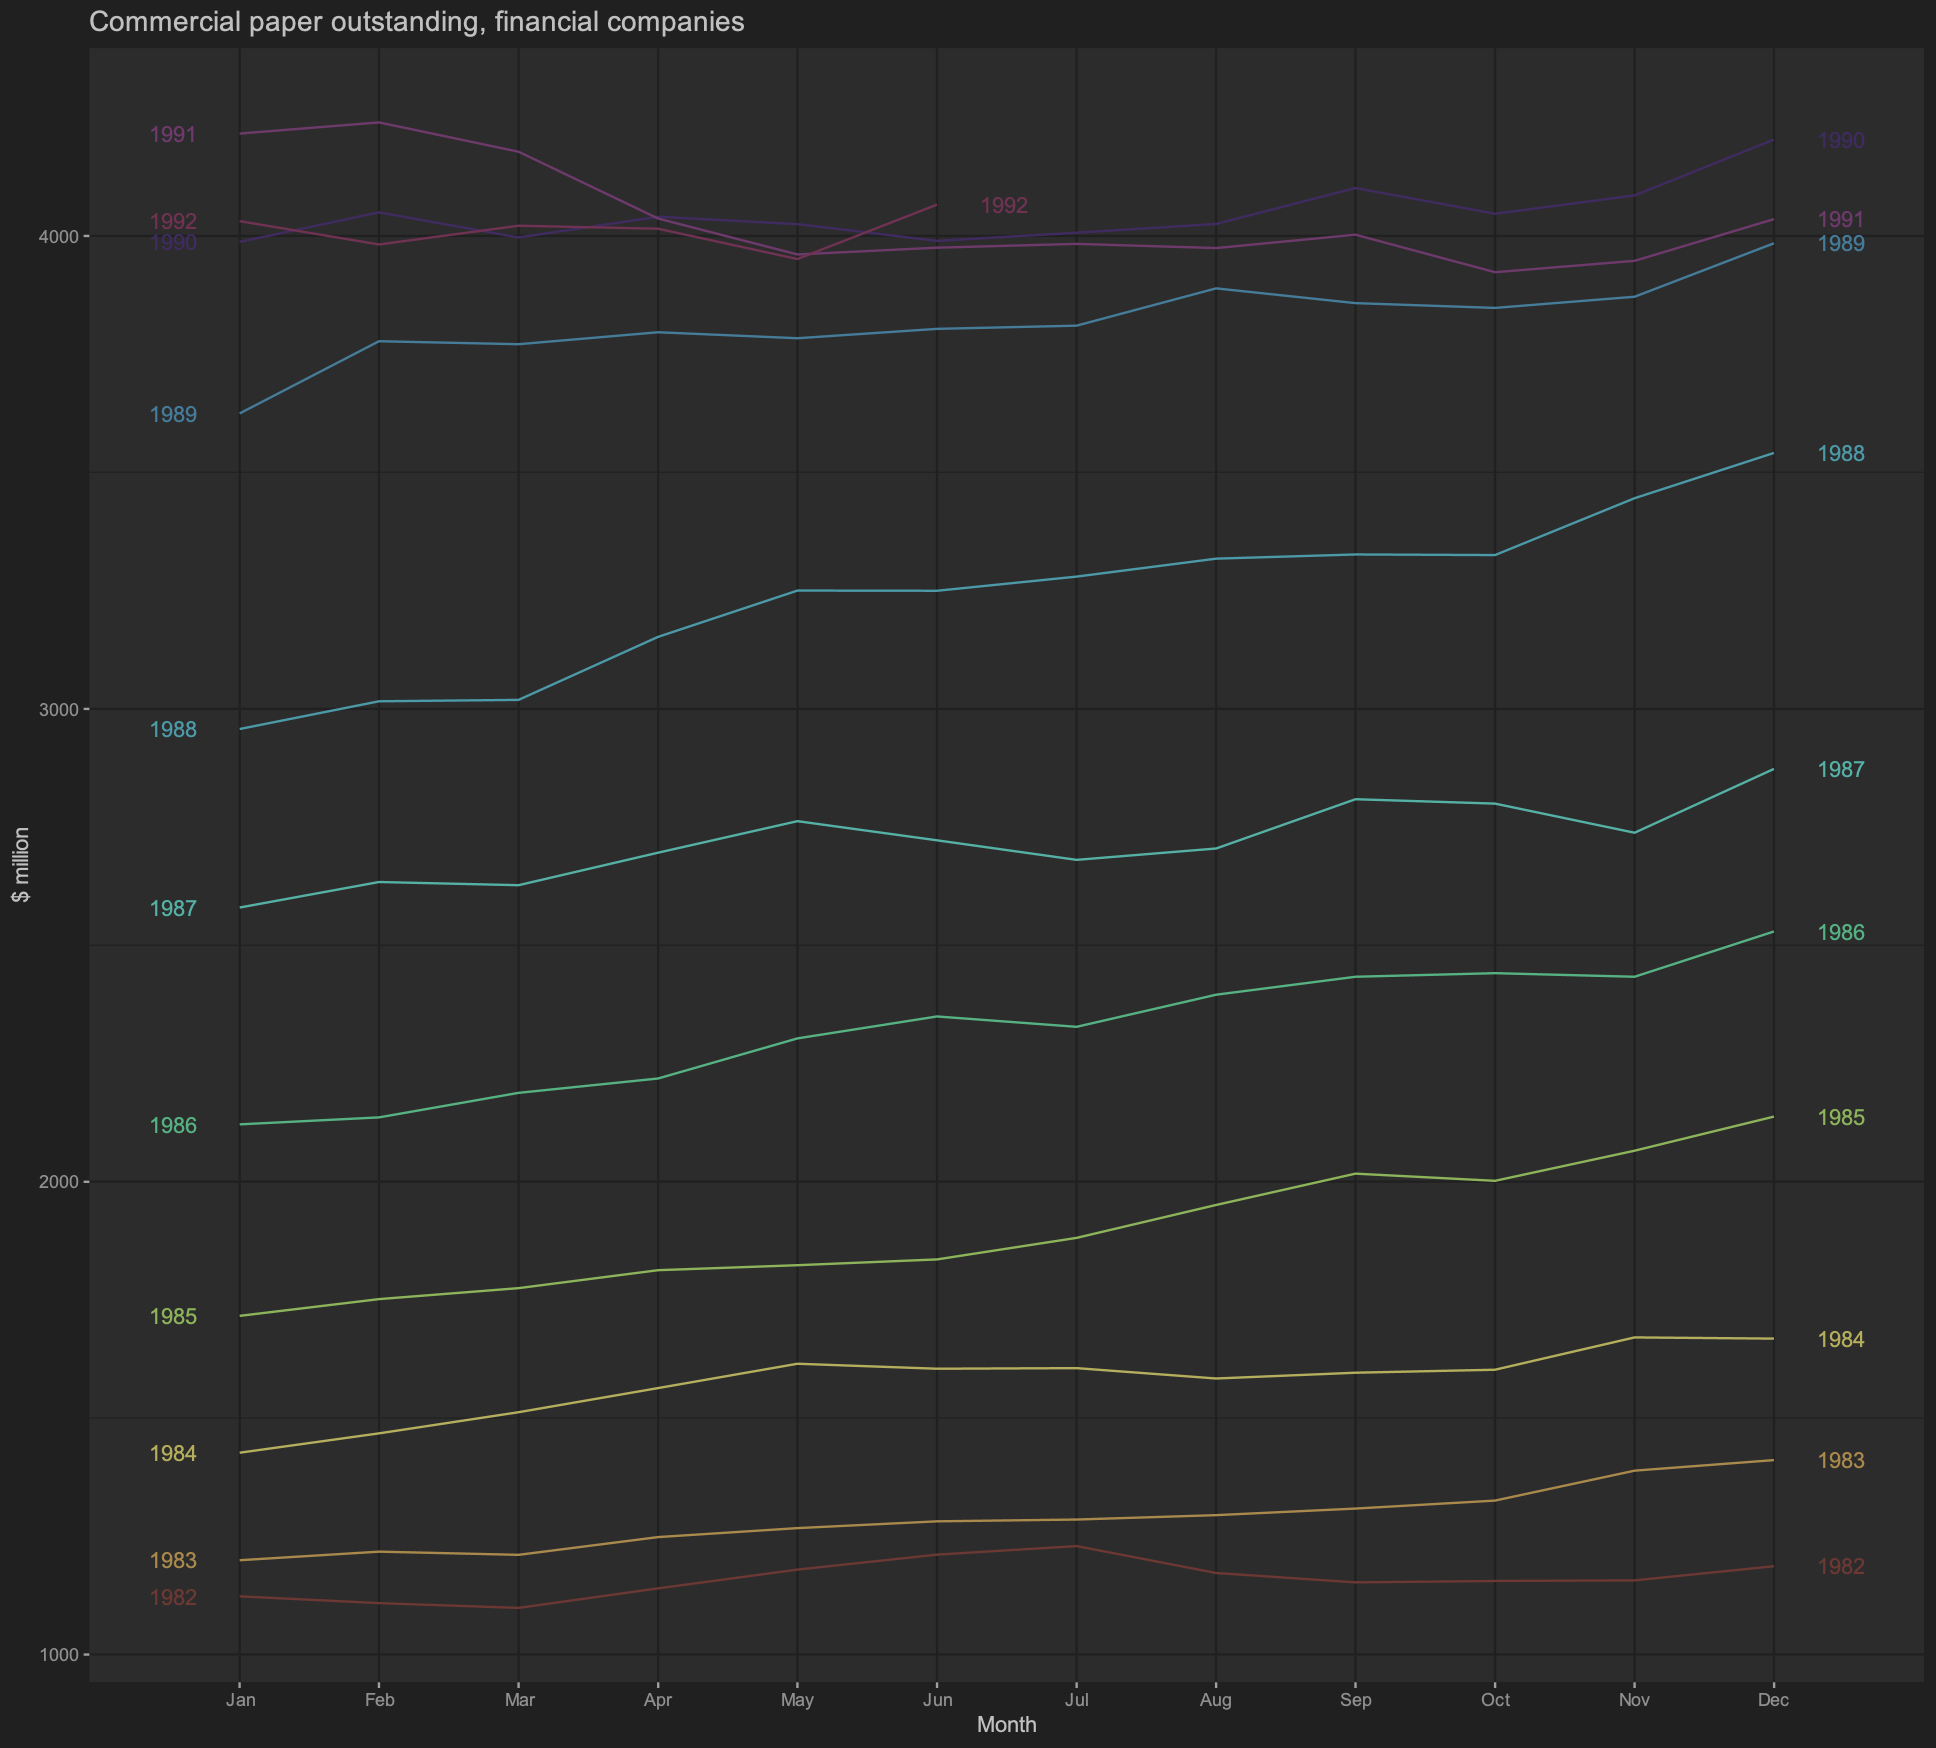
\includegraphics[width=.95\linewidth]{seasonplot}
    \caption{Seasonal plot of the time series}
  \end{subfigure}%
  \begin{subfigure}{.5\textwidth}
  \centering
    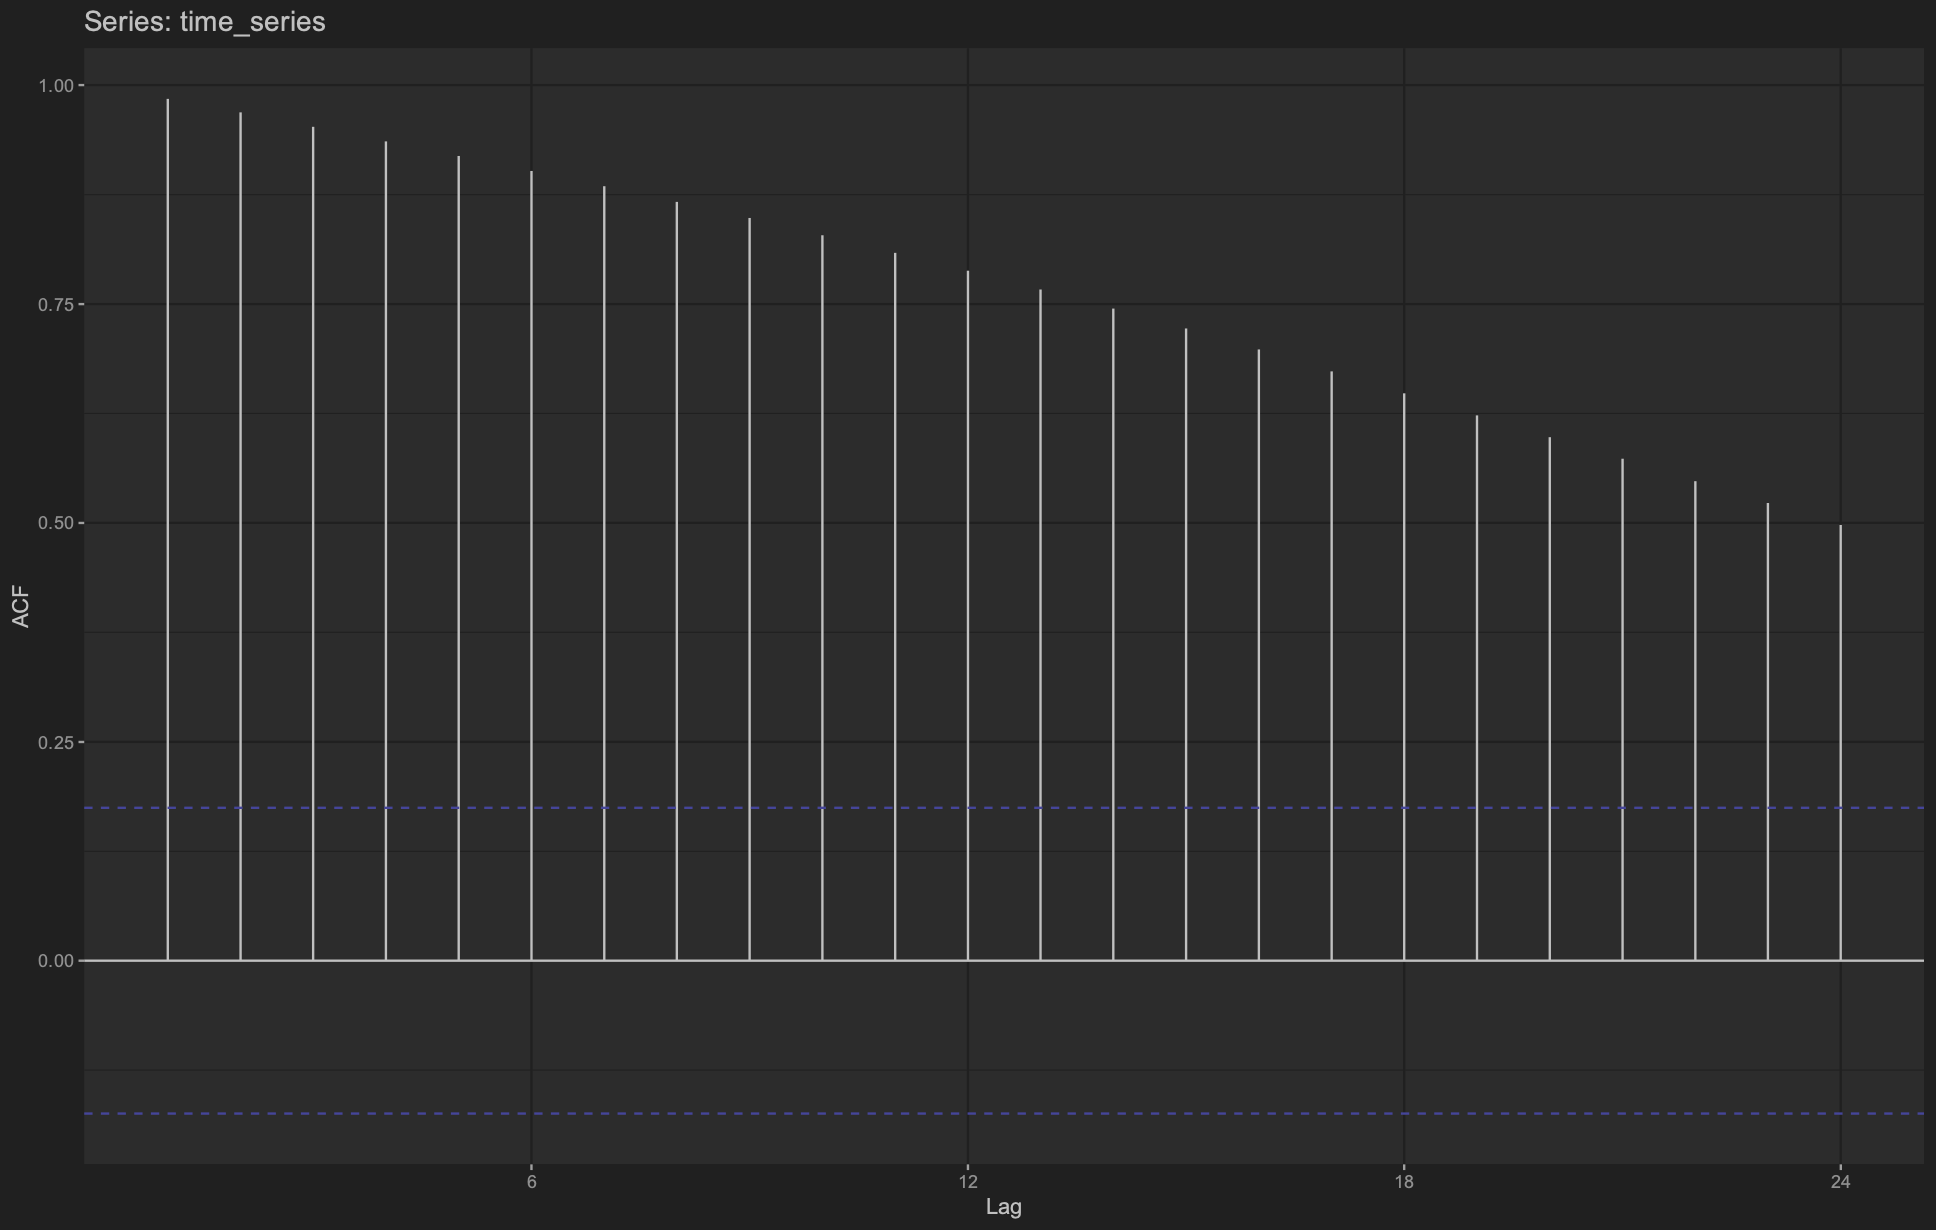
\includegraphics[width=.95\linewidth]{acf}
    \caption{Auto-correlation function of the time series}
  \end{subfigure}
  \caption{Exploratory analysis of the time series}
  \label{fig:sesaonplot}
\end{figure}
